
%Assignment 1:  problems 2, 4, 7, 11, 13, 22 on pages 27-29 of the course notes.

\documentclass{article}

\usepackage{amsmath}
\usepackage{amssymb}
\usepackage{graphicx}

\newcommand{\R}{\mathbb{R}}
\newcommand{\N}{\mathbb{N}}
\newcommand{\Z}{\mathbb{Z}}

\author{Jacob Errington}
\date{24 September 2014}
\title{Algebra I -- Assignment \#1}

\begin{document}

\maketitle

\section*{Problem \#2}

Compute the the set intersections and unions.

\begin{enumerate}
    \item Let $N \geq 0$. 
        
        \begin{enumerate}
            \item What is $\bigcup_{n=1}^N \left[-n,\,n\right]$ ?

                Since $[-n,\,n] \cup [-(n+1),\, n+1] = [-(n+1),\, n+1]$, the union of all
                these sets will simply be $[-N, N]$. In other words, since the next set
                is always a superset of the previous one, the union is simply the biggest
                set in the desired union.

            \item What is $\bigcap_{n=1}^N [-n, n]$ ?

                Since $[-n,\,n] \cap [-(n+1),\, n+1] = [-n,\, n]$, the union of all these
                sets will simply be $[-1, 1]$. In other words, that is the subset shared
                between all the sets in the desired intersection.
        \end{enumerate}

    \item Compute the infinite unions.
        
        \begin{enumerate}
            \item What is $\bigcup_{n=1}^\infty [n,\, n+1]$ ?

                Since $[n,\, n+1] \cup [n+1,\, n+2] = [n,\, n+2]$, the full union is 
                $[1, \infty)$.

            \item What is $\bigcup_{n=1}^\infty (n,\, n+2)$ ?

                The openness of these intervals is effectively excluding all the positive
                odd integers. Therefore, the full union is
                \begin{equation*}
                    \left\{ x \in \R,\, n \in \N^*: x > 1,\, x \neq 2n + 1 \right\}
                \end{equation*}
                where $\N^*$ represents the nonzero natural numbers.
        \end{enumerate}

    \item Compute the infinite unions.

        \begin{enumerate}
            \item What is $\bigcup_{n=1}^\infty (n,\, n+1)$ ?

                Here, all the nonzero naturals are excluded. The union is therefore
                \begin{equation*}
                    \left\{ x \in \R: x > 1\right\} \setminus \N^*
                \end{equation*}

            \item What is $\bigcup_{n=1}^\infty (\frac{1}{n},\, 1]$ ?

                Every subsequent set is a superset of all the previous sets, i.e. 
                $(\frac{1}{n+1},\, 1] \supset (\frac{1}{n},\, 1]$ for all $n \in \N^*$.
                Thus, the overall union is simply the interval as $n$ tends to infinity.
                \begin{equation*}
                    \lim_{n\to\infty} \left(\frac{1}{n}, 1\right] = \left(0, 1\right]
                \end{equation*}
        \end{enumerate}

    \item Let $A_n = \left\{ x^n : x \in \N \right\}$; what is 
        $\bigcap_{n=1}^\infty A_n$ ?

        We observe the following graphs of the polynomials in question to gain some
        intuition about the problem.

        \begin{figure}[h]
            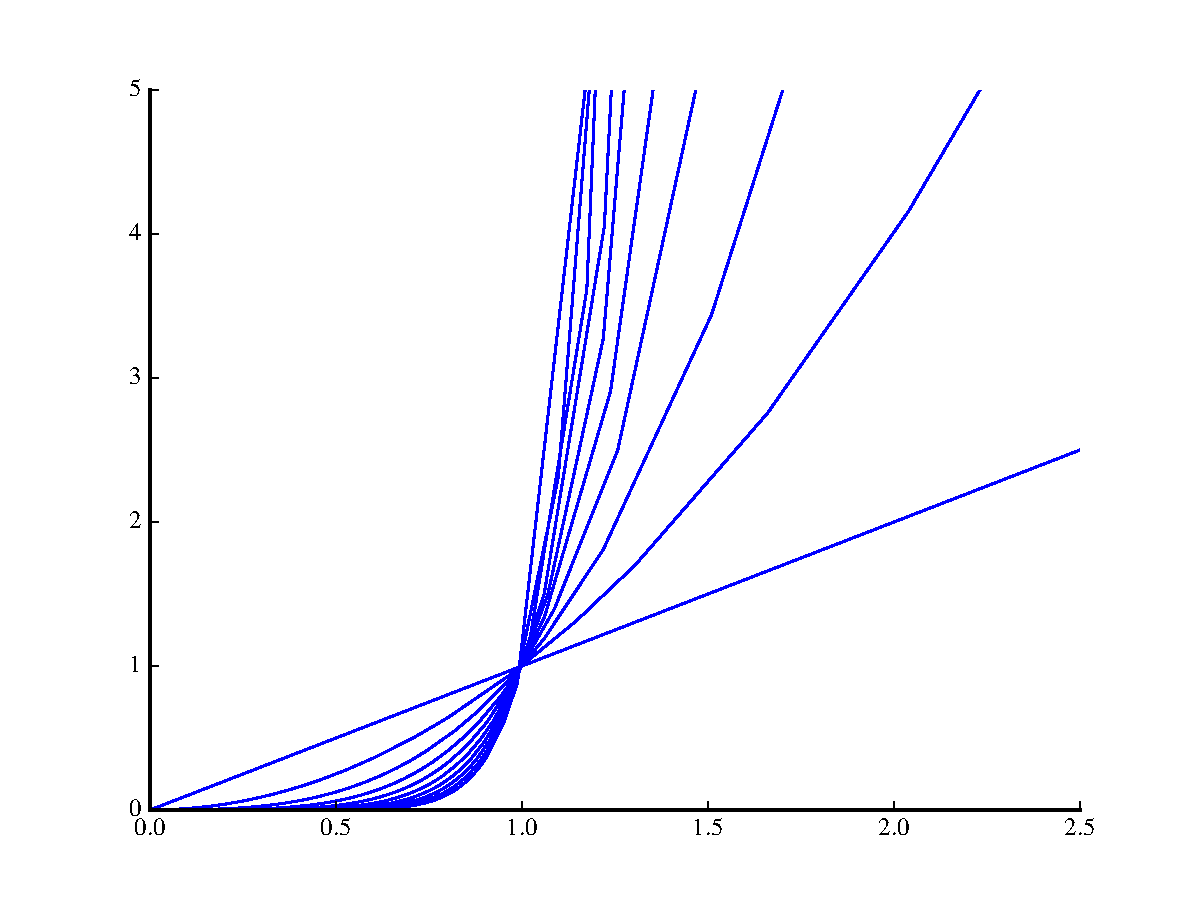
\includegraphics[width=\textwidth]{polynomials.pdf}
            \caption{The graphs of equations defined by the polynomials 
                $x^n,\, n \in \{1, ..., 10\}$}
        \end{figure}

        For $x \in \R,\, n,\, m \in \N$, $x = 0 \lor x = 1 \implies x^n = x^m$, and in
        the case where $x \in \N$, the implication is bidirectional. Thus, the
        intersection of $A_n$ is $\{0, 1\}$.

    \item Let $B_n = \left\{ (x, y) \in \R^2: y^n \leq x \right\}$

        \begin{enumerate}
            \item What is $\bigcup_{n=1}^\infty B_n$ ?

                This inequality geometrically refers to the region to the left of the
                curves. There are three problematic points where we must be careful:
                $x=-1,\, x=0,\, x=1$. 
                
                At $x=-1$, the line intersects with all the odd
                polynomials. 

            \item What is $\bigcap_{n=1}^\infty B_n$ ?
        \end{enumerate}
\end{enumerate}

\end{document}
